\chapter*{Proposition 8}
\label{prop:8}

\begin{figure*}[ht]
    \begin{center}
    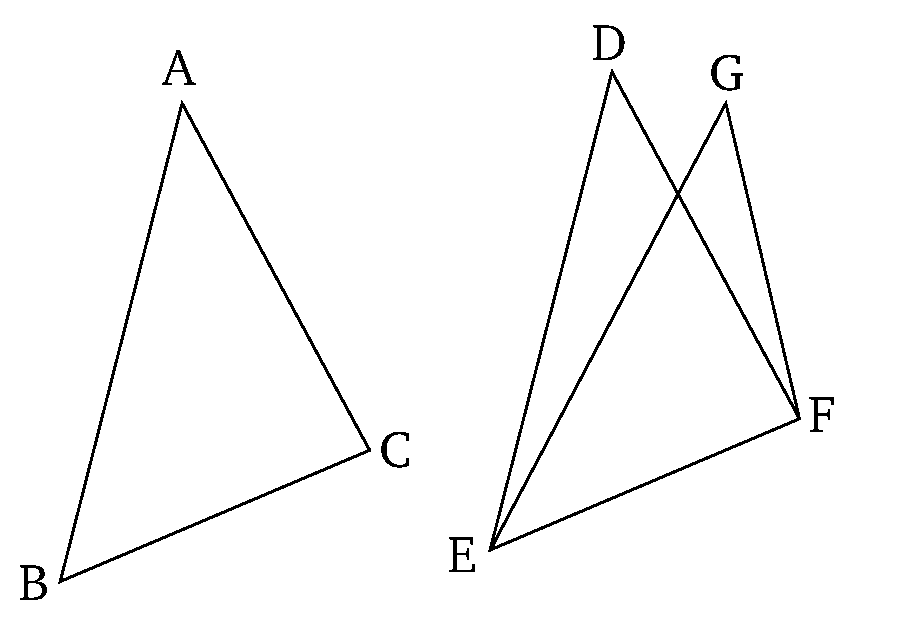
\includegraphics[width=0.5\linewidth]{figures/fig08e.eps}
    \label{fig:prop_8}
    \end{center}
\end{figure*}

If two triangles have  two sides equal to two sides, respectively, 
and also have the base equal to the base, then they will
also have equal the angles  encompassed by
the equal straight-lines.

Let $ABC$ and $DEF$ be two triangles having the two sides $AB$ and $AC$ equal to the two
sides $DE$ and $DF$, respectively. (That is) $AB$ to $DE$, and $AC$ to $DF$.  Let them also have
the base $BC$ equal to the base $EF$. I say that the angle $BAC$ is also equal
to the angle $EDF$.

For if triangle $ABC$ is applied to triangle $DEF$, the point $B$ being placed on
point $E$, and the straight-line $BC$ on $EF$, then point $C$ will also coincide with $F$, on
account of $BC$ being equal to $EF$.
So  (because of) $BC$ coinciding with $EF$,  (the sides) $BA$ and $CA$ will also
coincide with  $ED$ and $DF$ (respectively). 
For if base $BC$ coincides with base $EF$, but the sides $AB$ and $AC$ 
do not coincide with $ED$ and $DF$ (respectively), but miss like $EG$
and $GF$ (in the above figure), 
then we will have constructed upon the same straight-line, two other straight-lines equal, respectively, to two (given) straight-lines,  and (meeting)
at a different point on the same
side (of the straight-line), but having the same ends. But (such straight-lines) cannot be constructed [Prop.~1.7].
Thus,  the base $BC$ being applied to the  base $EF$,  the sides $BA$ and $AC$
cannot not coincide with $ED$ and $DF$ (respectively). Thus, they
will coincide. So the angle $BAC$ will also coincide with angle $EDF$,
and will be equal to it [C.N.~\ref{cn:4}].

Thus, if two triangles have  two  sides equal to two side, respectively,
and  have the base equal to the base, then they will also have equal the angles  encompassed by
the equal straight-lines. (Which is) the very thing it was required to show.


\section*{Commentary}

\begin{proposition}\label{proposition_8}\lean{Elements.Book1.proposition_8}\leanok
    $\triangle~ABC$ and $\triangle~DEF$ are two triangles with $AB = DE$, $AC = DF$, and $BC = EF$. Then, $\angle~BAC = \angle~EDF$.
\end{proposition}
\begin{proof}
    \uses{proposition_7}\leanok
    See the original proof by Euclid.
\end{proof}
